% Options for packages loaded elsewhere
\PassOptionsToPackage{unicode}{hyperref}
\PassOptionsToPackage{hyphens}{url}
%
\documentclass[
  ignorenonframetext,
  aspectratio=169,
]{beamer}
\usepackage{pgfpages}
\setbeamertemplate{caption}[numbered]
\setbeamertemplate{caption label separator}{: }
\setbeamercolor{caption name}{fg=normal text.fg}
\beamertemplatenavigationsymbolsempty
% Prevent slide breaks in the middle of a paragraph
\widowpenalties 1 10000
\raggedbottom
\setbeamertemplate{part page}{
  \centering
  \begin{beamercolorbox}[sep=16pt,center]{part title}
    \usebeamerfont{part title}\insertpart\par
  \end{beamercolorbox}
}
\setbeamertemplate{section page}{
  \centering
  \begin{beamercolorbox}[sep=12pt,center]{part title}
    \usebeamerfont{section title}\insertsection\par
  \end{beamercolorbox}
}
\setbeamertemplate{subsection page}{
  \centering
  \begin{beamercolorbox}[sep=8pt,center]{part title}
    \usebeamerfont{subsection title}\insertsubsection\par
  \end{beamercolorbox}
}
\AtBeginPart{
  \frame{\partpage}
}
\AtBeginSection{
  \ifbibliography
  \else
    \frame{\sectionpage}
  \fi
}
\AtBeginSubsection{
  \frame{\subsectionpage}
}

\usepackage{amsmath,amssymb}
\usepackage{lmodern}
\usepackage{iftex}
\ifPDFTeX
  \usepackage[T1]{fontenc}
  \usepackage[utf8]{inputenc}
  \usepackage{textcomp} % provide euro and other symbols
\else % if luatex or xetex
  \usepackage{unicode-math}
  \defaultfontfeatures{Scale=MatchLowercase}
  \defaultfontfeatures[\rmfamily]{Ligatures=TeX,Scale=1}
\fi
\usetheme[]{Madrid}
\usecolortheme{DarkBlue}
% Use upquote if available, for straight quotes in verbatim environments
\IfFileExists{upquote.sty}{\usepackage{upquote}}{}
\IfFileExists{microtype.sty}{% use microtype if available
  \usepackage[]{microtype}
  \UseMicrotypeSet[protrusion]{basicmath} % disable protrusion for tt fonts
}{}
\makeatletter
\@ifundefined{KOMAClassName}{% if non-KOMA class
  \IfFileExists{parskip.sty}{%
    \usepackage{parskip}
  }{% else
    \setlength{\parindent}{0pt}
    \setlength{\parskip}{6pt plus 2pt minus 1pt}}
}{% if KOMA class
  \KOMAoptions{parskip=half}}
\makeatother
\usepackage{xcolor}
\newif\ifbibliography
\setlength{\emergencystretch}{3em} % prevent overfull lines
\setcounter{secnumdepth}{-\maxdimen} % remove section numbering


\providecommand{\tightlist}{%
  \setlength{\itemsep}{0pt}\setlength{\parskip}{0pt}}\usepackage{longtable,booktabs,array}
\usepackage{calc} % for calculating minipage widths
\usepackage{caption}
% Make caption package work with longtable
\makeatletter
\def\fnum@table{\tablename~\thetable}
\makeatother
\usepackage{graphicx}
\makeatletter
\def\maxwidth{\ifdim\Gin@nat@width>\linewidth\linewidth\else\Gin@nat@width\fi}
\def\maxheight{\ifdim\Gin@nat@height>\textheight\textheight\else\Gin@nat@height\fi}
\makeatother
% Scale images if necessary, so that they will not overflow the page
% margins by default, and it is still possible to overwrite the defaults
% using explicit options in \includegraphics[width, height, ...]{}
\setkeys{Gin}{width=\maxwidth,height=\maxheight,keepaspectratio}
% Set default figure placement to htbp
\makeatletter
\def\fps@figure{htbp}
\makeatother

\definecolor{DarkBlue}{rgb}{0.05, 0.15, 0.3}
\setbeamercolor{structure}{fg=DarkBlue}
\makeatletter
\makeatother
\makeatletter
\makeatother
\makeatletter
\@ifpackageloaded{caption}{}{\usepackage{caption}}
\AtBeginDocument{%
\ifdefined\contentsname
  \renewcommand*\contentsname{Table of contents}
\else
  \newcommand\contentsname{Table of contents}
\fi
\ifdefined\listfigurename
  \renewcommand*\listfigurename{List of Figures}
\else
  \newcommand\listfigurename{List of Figures}
\fi
\ifdefined\listtablename
  \renewcommand*\listtablename{List of Tables}
\else
  \newcommand\listtablename{List of Tables}
\fi
\ifdefined\figurename
  \renewcommand*\figurename{Figure}
\else
  \newcommand\figurename{Figure}
\fi
\ifdefined\tablename
  \renewcommand*\tablename{Table}
\else
  \newcommand\tablename{Table}
\fi
}
\@ifpackageloaded{float}{}{\usepackage{float}}
\floatstyle{ruled}
\@ifundefined{c@chapter}{\newfloat{codelisting}{h}{lop}}{\newfloat{codelisting}{h}{lop}[chapter]}
\floatname{codelisting}{Listing}
\newcommand*\listoflistings{\listof{codelisting}{List of Listings}}
\makeatother
\makeatletter
\@ifpackageloaded{caption}{}{\usepackage{caption}}
\@ifpackageloaded{subcaption}{}{\usepackage{subcaption}}
\makeatother
\makeatletter
\@ifpackageloaded{tcolorbox}{}{\usepackage[many]{tcolorbox}}
\makeatother
\makeatletter
\@ifundefined{shadecolor}{\definecolor{shadecolor}{rgb}{.97, .97, .97}}
\makeatother
\makeatletter
\makeatother
\ifLuaTeX
  \usepackage{selnolig}  % disable illegal ligatures
\fi
\IfFileExists{bookmark.sty}{\usepackage{bookmark}}{\usepackage{hyperref}}
\IfFileExists{xurl.sty}{\usepackage{xurl}}{} % add URL line breaks if available
\urlstyle{same} % disable monospaced font for URLs
\hypersetup{
  pdftitle={6.3: Survival Analysis and Censored Data},
  pdfauthor={Navona Calarco},
  hidelinks,
  pdfcreator={LaTeX via pandoc}}

\title{6.3: Survival Analysis and Censored Data}
\author{Navona Calarco}
\date{}
\institute{The University of Toronto}

\begin{document}
\frame{\titlepage}
\ifdefined\Shaded\renewenvironment{Shaded}{\begin{tcolorbox}[interior hidden, breakable, boxrule=0pt, enhanced, borderline west={3pt}{0pt}{shadecolor}, frame hidden, sharp corners]}{\end{tcolorbox}}\fi

\begin{frame}{Introduction}
\protect\hypertarget{introduction}{}
Survival analysis and censored data are related to the analysis of the
outcome variable best described as ``the time until and event occurs''.
Some examples include:

\begin{itemize}
\item
  Predicting survival time of patients diagnosed with cancer.
\item
  Predicting the time a customer will cancel a subscription.
\item
  Predicting the customer wait time for a call centre.
\end{itemize}
\end{frame}

\begin{frame}{Survival and Censoring Times}
\protect\hypertarget{survival-and-censoring-times}{}
For each individual we assume there exists:

\begin{itemize}
\item
  \(T\): the true \textbf{survival time} which represents the time at
  which the event of interest occurs. ~~~~~\emph{Ex: The time at which
  the patient dies.}
\item
  \(C\): the true \textbf{censoring time} which is when the censoring
  occurs. ~~~~~~~~~\emph{Ex: The time at which the patient drops out of
  the study.}
\end{itemize}

However, we only ever observe the time that comes first:
\[Y=\min (T, C)\] In order to keep track of which time \(Y\) represents,
we also have a status indicator: \[
\delta=\left\{\begin{array}{ll}
1 & \text { if } T \leq C \\
0 & \text { if } T>C
\end{array}\right.\]
\end{frame}

\begin{frame}{Survival and Censoring Times}
\protect\hypertarget{survival-and-censoring-times-1}{}
Suppose we have the following data from a medical study with \(n = 4\)
patients. We observe 4 pairs of \((Y, \delta)\), denoted as
\((y_1, \delta_1), \dots, (y_4, \delta_4)\).

\begin{columns}[T]
\begin{column}{0.6\textwidth}
\begin{figure}

{\centering 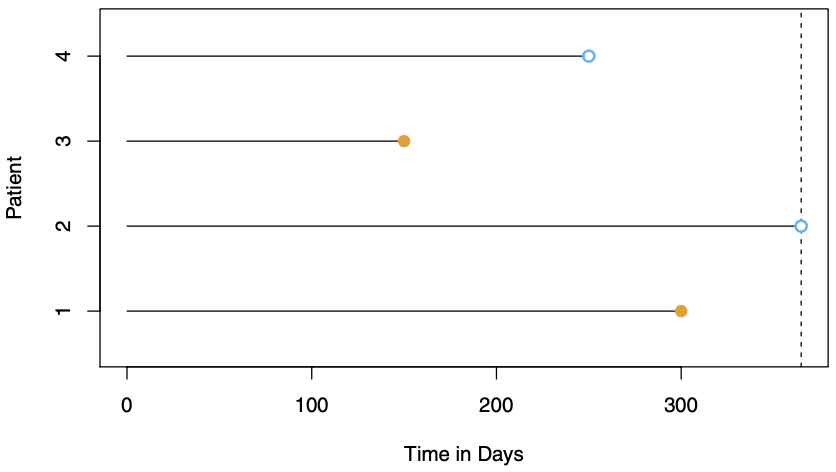
\includegraphics[width=3.22917in,height=\textheight]{images/patients_time.png}

}

\end{figure}
\end{column}

\begin{column}{0.4\textwidth}
\begin{itemize}
\item
  For patient 1 and 3, we observe the time to the event (i.e.~death)
  during the study.

  \begin{itemize}
  \tightlist
  \item
    Thus, \(\delta_1 = \delta_3 = 1\)
  \end{itemize}
\item
  Patient 2 survives until the end of the study.

  \begin{itemize}
  \tightlist
  \item
    Thus, \(\delta_2 = 0\)
  \end{itemize}
\item
  Patient 4 drops out of the study early.

  \begin{itemize}
  \tightlist
  \item
    Thus, \(\delta_4 = 0\)
  \end{itemize}
\end{itemize}
\end{column}
\end{columns}
\end{frame}

\begin{frame}{Independent Censoring}
\protect\hypertarget{independent-censoring}{}
We assume that the censoring mechanism is independent. That is, the
\alert{event time $T$ is independent of the censoring time $C$}.

Example of a violation:

\begin{itemize}
\item
  Some patients drop out of a cancer study because they are very sick.
\item
  If we analyse the data without considering why patients drop out then
  we will overestimate the true average survival time.
\end{itemize}

The data collection process must be examined closely to check whether
independent censoring is a reasonable assumption.
\end{frame}

\begin{frame}{The Kaplan-Meier Survival Curve}
\protect\hypertarget{the-kaplan-meier-survival-curve}{}
The Kaplan-Meier survial curve (or survival function) is a decreasing
function that
\alert{quantifies the probability of surviving past time $t$}. It is
defined by \[S(t)=\operatorname{Pr}(T>t)\] Estimating \(S(t)\) is
complicated by the presence of censoring but we have an approach to
overcome this challenge.

\begin{itemize}
\item
  \(d_{1}<d_{2}<\cdots<d_{K}\) denote the \(K\) unique survival times
  among the non-censored individuals.
\item
  \(q_k\) denotes the number of events that took place at time \(d_k\).
  (i.e.~the number of patients that died at time \(d_k\))
\item
  \(r_k\) denotes the number of individuals alive and in the study just
  before \(d_k\) (the \textbf{at risk} patients).
\item
  The set of patients that are at risk are the \textbf{risk set}.
\end{itemize}
\end{frame}

\begin{frame}{The Kaplan-Meier Survival Curve}
\protect\hypertarget{the-kaplan-meier-survival-curve-1}{}
So, the probability of surviving past time \(d_k\) is given by: \[
S\left(d_{k}\right)=\operatorname{Pr}\left(T>d_{k}\right)=\operatorname{Pr}\left(T>d_{k} \mid T>d_{k-1}\right) \operatorname{Pr}\left(T>d_{k-1}\right).
\] Note that \(\operatorname{Pr}\left(T>d_{k-1}\right)\) amounts to
\(S\left(d_{k-1}\right)\). So,
\[S\left(d_{k}\right)=\operatorname{Pr}\left(T>d_{k} \mid T>d_{k-1}\right) S\left(d_{k-1}\right).\]
Thus, \[
S\left(d_{k}\right)=\operatorname{Pr}\left(T>d_{k} \mid T>d_{k-1}\right) \times \cdots \times \operatorname{Pr}\left(T>d_{2} \mid T>d_{1}\right) \operatorname{Pr}\left(T>d_{1}\right)
\] Now we need the estimates for each of these terms.
\end{frame}

\begin{frame}{The Kaplan-Meier Survival Curve}
\protect\hypertarget{the-kaplan-meier-survival-curve-2}{}
The estimator \[
\widehat{\operatorname{Pr}}\left(T>d_{j} \mid T>d_{j-1}\right)=\left(r_{j}-q_{j}\right) / r_{j}
\] is the fraction of the risk set at time \(d_j\) who survived past
time \(d_j\). So, the \textbf{Kaplan-Meier estimator} of the survival
curve is
\[\widehat{S}\left(d_{k}\right)=\prod_{j=1}^{k}\left(\frac{r_{j}-q_{j}}{r_{j}}\right)\]

\begin{itemize}
\item
  For times \(t\) between \(d_k\) and \(d_{k+1}\) we set
  \(\widehat{S}(t)=\widehat{S}\left(d_{k}\right)\).
\item
  This gives the Kaplan-Meier survival curve a step-like shape.
\end{itemize}
\end{frame}

\begin{frame}{Exercise: The Kaplan-Meier Survival Curve}
\protect\hypertarget{exercise-the-kaplan-meier-survival-curve}{}
Open the Survival Analysis and Censored Data R Markdown file.

\begin{itemize}
\tightlist
\item
  Go over the ``The Kaplan-Meier Survival Curve'' section together as a
  class.
\end{itemize}
\end{frame}

\begin{frame}{The Log-Rank Test}
\protect\hypertarget{the-log-rank-test}{}
The log-rank test aims to test the null hypothesis that there is no
difference between two survival curves. The statistic is computed with
\[W=\frac{X-\mathrm{E}(X)}{\sqrt{\operatorname{Var}(X)}}\] where
\(\mathrm{E}(X)\) and \(\operatorname{Var}(X)\) are the expectation and
variance under the assumption of the null hypothesis.
\end{frame}

\begin{frame}{The Log-Rank Test\}}
\protect\hypertarget{the-log-rank-test-1}{}
Suppose we want to \alert{compare the survival of two groups of people}
by comparing the two survival curves.

Recall:

\begin{itemize}
\item
  \(d_{1}<d_{2}<\cdots<d_{K}\) are the unique survival times among the
  non-censored individuals.
\item
  \(r_k\) is the number of individuals at risk at time \(d_k\).
\item
  \(q_k\) denotes the number of patients that died at time \(d_k\)
\end{itemize}

Now we define:

\begin{itemize}
\item
  \(r_{1k}, r_{2k}\) are the number of individuals at risk at time
  \(d_k\) in group 1 and 2 respectively.
\item
  \(q_{1k}, q_{2k}\) are the number of patients that died at time
  \(d_k\) in group 1 and 2 respectively.
\item
  Note that \(r_{1 k}+r_{2 k}=r_{k}\) and \(q_{1 k}+q_{2 k}=q_{k}\).
\end{itemize}
\end{frame}

\begin{frame}{The Log-Rank Test}
\protect\hypertarget{the-log-rank-test-2}{}
At each death time \(d_k\), we have the following table:

\begin{center}
\begin{tabular}{l|cc|c} 
& Group 1 & Group 2 & Total \\
\hline Died & $q_{1 k}$ & $q_{2 k}$ & $q_{k}$ \\
Survived & $r_{1 k}-q_{1 k}$ & $r_{2 k}-q_{2 k}$ & $r_{k}-q_{k}$ \\
\hline Total & $r_{1 k}$ & $r_{2 k}$ & $r_{k}$
\end{tabular}
\end{center}

\begin{itemize}
\item
  \(\frac{r_{1 k}}{r_{k}}\) is the proportion of at risk individuals
  that are in group 1.
\item
  If there is no difference in the survival rate between the two groups,
  we would expect \(\frac{r_{1 k}}{r_{k}}q_{k}\) individuals in group 1
  to die at time \(d_k\).
\item
  So, \(\mathrm{E}\left(q\_{1 k}\right)=\frac{r_{1 k}}{r_{k}} q\_{k}\)
  is the expected number of deaths at time \(d_k\) in group 1.
\end{itemize}
\end{frame}

\begin{frame}{The Log-Rank Test}
\protect\hypertarget{the-log-rank-test-3}{}
In our case, the log rank test statistic is computed with \[
W=\frac{\sum_{k=1}^{K}\left(q_{1 k}-\mathrm{E}\left(q_{1 k}\right)\right)}{\sqrt{\sum_{k=1}^{K} \operatorname{Var}\left(q_{1 k}\right)}}
\] where \[
\operatorname{Var}\left(q_{1 k}\right)=\frac{q_{k}\left(r_{1 k} / r_{k}\right)\left(1-r_{1 k} / r_{k}\right)\left(r_{k}-q_{k}\right)}{r_{k}-1}.
\]

\begin{itemize}
\item
  When the sample size is large, \(W\) has approximately a standard
  normal distribution.
\item
  Then, a \(p\)-value can be used to test the null hypothesis that there
  is no difference between the survival curves of the two groups.
\end{itemize}
\end{frame}

\begin{frame}{Exercise: The Log-Rank Test}
\protect\hypertarget{exercise-the-log-rank-test}{}
Open the Survival Analysis and Censored Data R Markdown file.

\begin{itemize}
\tightlist
\item
  Go over the ``The Log-Rank Test'' section together as a class.
\end{itemize}
\end{frame}

\begin{frame}{Regression with a Survival Response}
\protect\hypertarget{regression-with-a-survival-response}{}
Suppose we would like to fit a regression model to survival data with
the following properties.

\begin{itemize}
\item
  \(n\) observations \((Y, \delta)\)

  \begin{itemize}
  \item
    \(Y = \min (T, C)\).
  \item
    \(\delta\) equals 1 if \(Y = T\) and 0 otherwise.
  \end{itemize}
\item
  \(X \in \mathbb{R}^p\) is a vector of \(p\) features.
\item
  We want to predict the true survival time \(T\).
\end{itemize}

Note that we want to predict \(T\), not \(Y\). Censoring makes this
difficult so we make use of the \textbf{hazard function}.
\end{frame}

\begin{frame}{The Hazard Function}
\protect\hypertarget{the-hazard-function}{}
The hazard function \(h(t)\) is
\alert{the death rate in the instant after time $t$, given survival past that time}.
That is,
\[h(t)=\lim _{\Delta t \rightarrow 0} \frac{\operatorname{Pr}(t<T \leq t+\Delta t \mid T>t)}{\Delta t}\]
where \(T\) is the unobserved survival time. We take the limit as
\(\Delta t\) approached zero so we can think of \(\Delta t\) as an
extremely small number.

Now we want to use the hazard function to model the survival time as a
function of the covariates \(x_{ij}\).
\end{frame}

\begin{frame}{The Proportional Hazards Assumption}
\protect\hypertarget{the-proportional-hazards-assumption}{}
The \textbf{proportional hazards assumption} states
\[h\left(t \mid x_{i}\right)=h_{0}(t) \exp \left(\sum_{j=1}^{p} x_{i j} \beta_{j}\right)\]

\begin{itemize}
\item
  \(h_0 (t) \geq 0\) is an unspecified function known as the
  \textbf{baseline hazard} which is the hazard function for an
  individual with features \(x_{i 1}=\cdots=x_{i p}=0\).
\item
  \(\exp \left(\sum_{j=1}^{p} x_{i j} \beta_{j}\right)\) is called the
  \textbf{relative risk} for the feature vector
  \(x_{i}=\left(x_{i 1}, \ldots, x_{i p}\right)\) relative to
  \(x_{i}=(0, \ldots, 0)\).
\end{itemize}

-\(\beta=\left(\beta_{0}, \beta_{1}, \ldots, \beta_{p}\right)\) are the
parameters that we need to estimate using the likelihood (we will not
present the likelihood function).
\end{frame}

\begin{frame}{The Proportional Hazards Assumption}
\protect\hypertarget{the-proportional-hazards-assumption-1}{}
Since the baseline hazard function \(h_0(t)\) is unspecified the only
assumption we are making is that a
\alert{one-unit increase in $x_{ij}$ corresponds to an increase in $h(t|x_i)$ by a factor of $\exp \left(\beta_{j}\right)$}.

\begin{columns}[T]
\begin{column}{0.7\textwidth}
\begin{figure}

{\centering 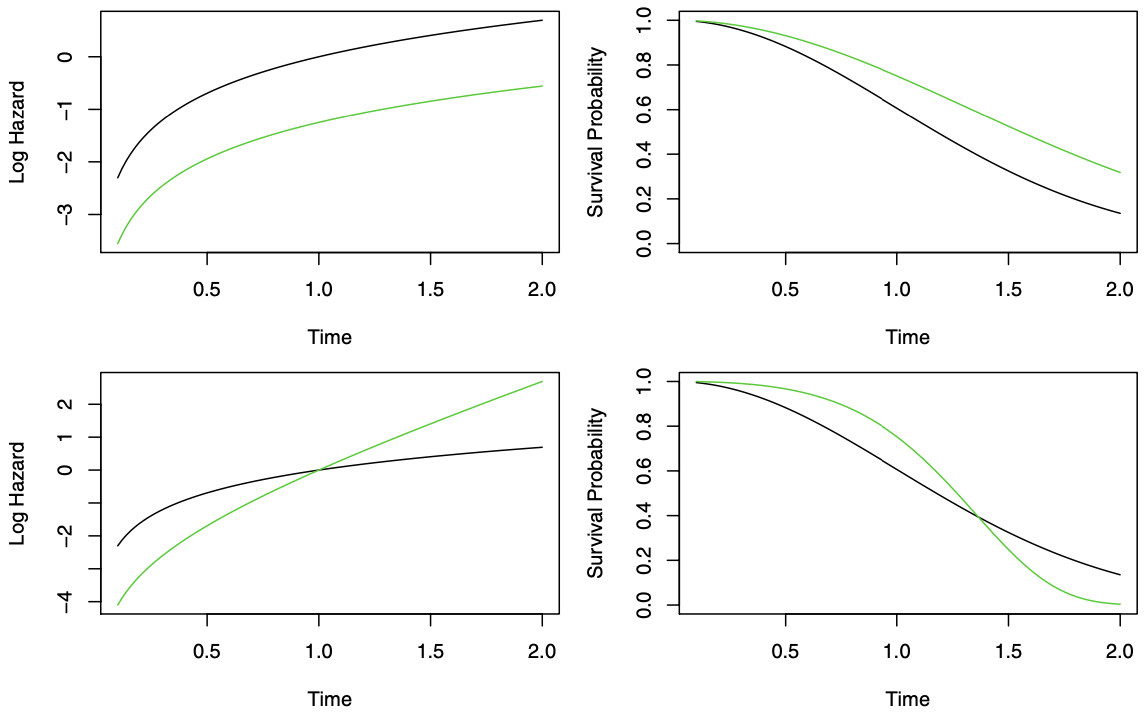
\includegraphics[width=4.17708in,height=\textheight]{images/proportional_assumption.png}

}

\end{figure}
\end{column}

\begin{column}{0.3\textwidth}
\begin{itemize}
\item
  Two models with a binary covariate \(x_i\).
\item
  Left plots show the log hazards and right plots show the survival
  functions.
\item
  Green is for \(x_i = 0\) and black is for \(x_i = 1\).
\item
  Top model satisfies the assumption.
\item
  Bottom model doesn't satisfy the assumption.
\end{itemize}
\end{column}
\end{columns}
\end{frame}

\begin{frame}{Cox Proportional Hazards Model}
\protect\hypertarget{cox-proportional-hazards-model}{}
Because \(h_0(t)\) in the proportional hazards assumption is unknown we
cannot plug \(h(t|x_i)\) into the likelihood to get estimates for
\(\beta=\left(\beta_{1}, \ldots, \beta_{p}\right)\).

\alert{Cox's proportional hazards model says that it it possible to estimate $\beta$ without specifying the form of $h_0(t)$.}

\begin{itemize}
\item
  Use the \textbf{partial likelihood} which is valid regardless of the
  the value of \(h_0(t)\).
\item
  Maximize the partial likelihood with respect to \(\beta\).
\item
  We can obtain \(p\)-values corresponding to null hypotesis such as
  \(H_0: \beta_j = 0\).
\item
  We can obtain confidence intervals associated with the estimated
  coefficients.
\end{itemize}
\end{frame}

\begin{frame}{Cox Proportional Hazards Model}
\protect\hypertarget{cox-proportional-hazards-model-1}{}
Suppose we have a single binary predictor \(x_i \in \{0, 1\}\) and we
want to determine whether there is a difference between the survival
times of the observations in the two groups.

\begin{itemize}
\item
  \emph{Approach \#1:} Fit a Cox proportional hazards model and test the
  null hypothesis \(H_0: \beta = 0\).
\item
  \emph{Approach \#2:} Perform a log-rank test to compare the two
  groups.
\end{itemize}

In the case of a binary predictor both methods will yield the same
result!
\end{frame}

\begin{frame}{Exercise: The Cox Proportional Hazards Model}
\protect\hypertarget{exercise-the-cox-proportional-hazards-model}{}
Open the Survival Analysis and Censored Data R Markdown file.

\begin{itemize}
\tightlist
\item
  Go over the ``The Cox Proportional Hazards Model'' section together as
  a class.
\end{itemize}
\end{frame}

\begin{frame}{References}
\protect\hypertarget{references}{}
Chapter 11 of the ISLR2 book:

James, Gareth, et al.~``Survival Analysis and Censored Data.'' An
Introduction to Statistical Learning: with Applications in R, 2nd ed.,
Springer, 2021.
\end{frame}



\end{document}
